\documentclass[a4paper,11pt,titlepage]{article}
\usepackage[T1]{fontenc}
\usepackage[utf8]{inputenc}
\usepackage{lmodern}
\usepackage[french]{babel}
\usepackage{graphicx}
\usepackage{color}
\usepackage{hyperref}
\usepackage{listings}
\usepackage{pgfplots}
\usepackage{tabularx}
\usepackage{xcolor}

\newcolumntype{C}{>{\centering\arraybackslash}X}

\hypersetup{
    colorlinks=true, % make the links colored
    linkcolor=blue, % color TOC links in blue
    urlcolor=gray, % color URLs in red
    linktoc=all % 'all' will create links for everything in the TOC
}

\lstset{
  basicstyle=\ttfamily,
  captionpos=b,
  language=c,
  frame=single,
  breaklines=true,
  upquote=true,
  commentstyle=\color{mygreen},
  prebreak=\space\textbackslash
}

\title{Rapport projet électronique}
\author{Rémi BOURGEON\\
\texttt{remi.bourgeon@isen.yncrea.fr}\\\\
Rodolphe HOUDAS\\
\texttt{rodolphe.houdas@isen.yncrea.fr}}
\date{2017-2018}

\begin{document}

\maketitle
\tableofcontents
\newpage

%\begin{abstract}
%\end{abstract}

\section{Description du projet}

\section{Choix de la résistance de gain}

L'amplificateur d'instrumentation INA118 utilise une résistance entre ses bornes $1$ et $8$ pour sélectionner le gain. Nos mesures nous ont permis de trouver que la cellule de pesée renvoie $5mV$ à charge pleine. Pour couvrir la plage de 0 à 5V de l'entrée analogique, nous avions besoin d'un gain de 1000. La datasheet de l'INA118 nous indique qu'il nous faut une résistance de 50$\Omega$ pour un gain de 1000.

\section{De l'utilisation du microcontrôleur}
Le montage conçu pour le projet utilise le microcontrôleur 8 bits PIC18F46K22.
Le microcontrôleur vient remplir le rôle d'orchestrateur entre les fonctionnalités du montage. En effet, il faut au moins un microcontrôleur pour contrôler l'écran LCD. Le PIC est aussi dôté d'un CAN (Convertisseur Analogique Numérique), ce qui lui permet de récupérer le signal renvoyé par la cellule de pesée et de pouvoir le numériser sur 8 ou 10 bits.
\subsection{Pourquoi ce PIC en particulier}
La première question que nous nous sommes posés a été de comprendre pourquoi ce PIC avait été sélectionné alors que nous en avions utilisé un autre durant les séances de TP.
D'abord il faut justifier l'évidence qui est qu'on a sélectionné un PIC18 plutôt qu'un microcontrôleur d'une autre marque (ou qu'un microcontrôleur 16 bits) pour des raisons de facilité. Nous avions de l'expérience avec les microcontrôleurs de cette gamme et par conséquent cela nous permettait de réutiliser nos connaissances et les bouts de programme dont nous disposions déjà, ce que nous avons fait.

En revanche, il n'était pas évident de comprendre pourquoi on utilisait le PIC18F46K22 plutôt que le PICF45K20 que nous avions utilisé en TP. La raison apparente est que les PICs du TP étaient déjà montés sur des cartes de prototypage, avec LEDs, potentiomètres, interrupteurs, etc. Cette carte était donc utile pour tester aisément les différentes fonctionnalités du PIC, mais ne permettait pas d'utiliser le PIC à d'autres fins. Nous disposions donc de ce que Microchip appelle la "Demo board", soit une carte de composants accompagnée d'un PIC pour explorer les fonctionnalités des PICs et prototyper quelques fonctionnalités simples sur les emplacements de prototypage. Cependant les pattes étant soudées à la carte, il n'y a pas vraiment moyen de changer la destination des différentes entrées et sorties.
Ceci étant dit, les PICF45K20 existent sans carte de démonstration, donc M. Lambert aurait pu les sélectionner pour le projet.
En comparant les prix, on se rend compte que le PIC18F46K22 est plus cher que le PIC18F45K20 (2,69 € vs. 1,86 € pour dizaine de microcontrôleurs). Donc si le prix ne justifie pas le choix de ce modèle, c'est qu'il doit avoir des caractéristiques intrinsèques différentes. Après examination attentive des premières pages de la datasheet des deux microcontrôleurs, je suis arrivé à déterminé que la seule différence dans les caractéristiques significatives était la consommation de courant ( < 20 nA en veille pour le modèle choisi vs. < 100 nA pour le modèle de TP).
Ce choix se justifie notamment parce que la destination du PIC sera d'être utilisé dans un montage avec une pile 9 V. Par conséquent un montage consommant cinq fois moins revient à proposer cinq fois plus d'autonomie. 

\section{Rôle du potentiomètre}
Le potentiomètre est une résistance variable. Elle est branchée sur la patte V0 de l'écran LCD, ce qui correspond à l'ajustement du contraste. En faisant rentrer une référence plus ou moins importante sur cette patte, l'écran va afficher un fond pour les caractères qui va être plus ou moins intense. Le potentiomètre est donc là pour permettre un ajustement du contraste.
\begin{figure}
  \begin{center}
    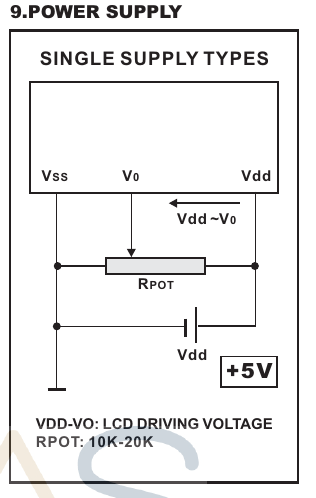
\includegraphics{./img/LCD_Supply.png}
    \caption{Fig 1. : Extrait de la datasheet de l'écran LCD}
    \label{fig:}
  \end{center}
\end{figure}

\section{Rôle du régulateur de tension}
Le régulateur de tension permet de convertir une tension délivrée par une pile 9 V en 5 V, ce qui est la tension acceptée par le PIC, le LCD et l'INA.


\section{Bits de configuration}

Conformément a ce qui avait été fait lors des TP d'électronique numérique, nous avons changé les bits de configuration suivants:\\

\begin{lstlisting}
FOSC  INTIO7
WDTEN OFF
LVP   OFF
\end{lstlisting}

Nous réglons l'horloge à 4Mhz à l'aide du registre \texttt{OSCCON} :\\

% Ok ici on a un bon tableau
% Le noindent est pour enlever l'indentation (sinon le tableau déborde dans l'autre sens
% Ici on utilise tabularx qui est une version améliorée de tabular
% |*{8}{C|} signifie qu'on crée 8 colonnes avec un bord (d'où le |) et dont le contenu est centré
\noindent
\begin{tabularx}{\textwidth}{|c|C|C|C|c|c|C|C|}
  \hline
  \multicolumn{8}{|>{\hsize=8\hsize}c|}{\texttt{OSCCON}}\\
  \hline
  % Ici on met le contenu des bits
  0 & 1 & 0 & 1 & 0 & 0 & 1 & 0\\
  \hline
  % Et ici les explications
  X 
  & \multicolumn{3}{>{\hsize=3\hsize}C|}{Horloge à 4Mhz} 
  & X & X 
  & \multicolumn{2}{>{\hsize=2\hsize}C|}{Utilisation de l'horloge interne}\\
  \hline
\end{tabularx}\\

Et on règle les interruptions:\\

\noindent
\begin{tabularx}{\textwidth}{|C|C|c|C|c|c|c|c|}
  \hline
  \multicolumn{8}{|>{\hsize=8\hsize}c|}{\texttt{INTCON}}\\
  \hline
  % Ici on met le contenu des bits
  1 & 1 & X & 1 & X & X & X & X\\
  \hline
  % Et ici les explications
  Activation des interruptions globales 
  & Activation des interruptions périphériques
  & X
  & Activation de l'interruption sur INT0
  & X & X & X & X\\
  \hline
\end{tabularx}\\\\

\noindent
\begin{tabularx}{\textwidth}{|C|C|c|c|c|c|c|c|}
  \hline
  \multicolumn{8}{|>{\hsize=8\hsize}c|}{\texttt{INTCON2}}\\
  \hline
  % Ici on met le contenu des bits
  1 & 0 & X & X & X & X & X & X\\
  \hline
  % Et ici les explications
  Interruption sur front descendant
  & \textit{À compléter}
  & X & X & X & X & X & X\\
  \hline
\end{tabularx}\\

\section{Application de la tare}

Une tare peut être prise lors de l'appui sur le bouton. Celui-ci est relié à une pin capable de déclencher une interruption matérielle pour exécuter une routine.\\

\begin{lstlisting}
HIGH_ISR
    ; Reinitialise le bit dinterruption
    BCF INTCON, 1
    CALL TARE
    RETFIE  FAST
\end{lstlisting}

La routine de tare prend une mesure de l'entrée analogique et enregistre la valeur brute dans un registre mémoire.\\

\begin{lstlisting}
TARE
    CALL ACQUISITION
    MOVFF RESULTLO, DEAD_WEIGHT
    RETURN
\end{lstlisting}

Cette valeur sera soustraite à la valeur mesurée avant conversion et affichage du poids.\\

\begin{lstlisting}
SHOWACQ
    CALL CLEARDISPLAY
    CALL ACQUISITION      ; Recuperation du poids (valeur brute)
    MOVF DEAD_WEIGHT, 0   
    SUBWF RESULTLO, 1     ; Application de la tare
\end{lstlisting}

\section{Application d'un coefficient correcteur}

La tension de sortie de la cellule de pesée est linéaire. À l'aide de différents poids, nous avons mesuré et placé sur un graphe les valeurs retournées par le CAN. À ce graphe, nous avons rajouté les valeurs que nous attendions (500 pour 500 grammes par exemple). On peut rapidement voir, à première vue, que la pente provenant du CAN doit être corrigée pour obtenir la même pente que le poids réel. Pour approximer la pente du CAN, nous avons calculé les pentes entre chaque segments puis nous avons fait la moyenne de ceux-ci. Nous avons supprimé une partie des dernières mesures, celles-ci paraissant fausses.\\

\begin{tikzpicture}
\begin{axis}
\addplot table [x=Weight, y=CAN output, col sep=comma] {../values.csv};
\addplot table [x=Weight, y=Weight, col sep=comma] {../values.csv};
\end{axis}
\end{tikzpicture}

Une fois la pente trouvée, nous avons pu calculer un coefficient correcteur à appliquer sur la valeur du CAN après suppression de la tare. Pour vérifier notre coefficient, nous avons calculé les valeurs corrigées. On peut observer une différence de maximum $\pm{2}$ grammes.\\

Comme nous ne pouvons pas multiplier par un nombre décimal en assembleur, nous devons multiplier à l'aide d'une fraction qui s'approche le plus possible du coefficient correcteur. En assembleur, pour multiplier par une fraction, il faut multiplier par le numérateur puis faire une division euclidienne par le dénominateur. Comme on multiplie par le numérateur, il faut veiller à ne pas utiliser de valeurs trop élevées pour que la valeur maximum ne déborde pas au-delà des 2 octets disponibles.\\

Nous avons calculé un coefficient correcteur de 1,07954. En arrondissant à 1,08, nous pouvons effectuer la conversion à l'aide d'une fraction $\frac{27}{25}$, ce qui nous permet de rester dans la gamme des valeurs disponibles ($1023 * 27 = 27621$)\\

\section{Problèmes rencontrés}

Lors du premier branchement de la cellule de pesée sur l'oscilloscope, nous n'arrivions pas à observer un changement de tension significatif. Nous avons donc rapidement monté la cellule de pesée sur un support permettant de la manipuler sans la maintenir gauchement sur un bord de table.\\

Une fois la cellule montée sur le support, nous avons pu aisément observer la variation de tension en fonction de la variation de poids et nous avons pu commencer à calculer le gain nécessaire.

Cependant, la cellule de pesée avait bien un comportement linéaire mais uniquement à plus de 60g sur le plateau. Au-dessus de 60g, chaque variation de tension apparaissait sur l'oscilloscope, même en rajoutant moins de 10g. En revanche, en-dessous de 60g, la cellule de pesée ne sortait aucune variation de tension. C'est la raison d'origine pour laquelle nous avions décidé de fixer la jauge sur un support : nous cherchions à avoir un montage mécanique plus stable pour arriver à détecter les petites variation de poids. En effet, les mesures des valeurs renvoyées par la cellule de pesée tenue à la main faisaient ressortir le même problème.

Nous avons donc fini par en parler avec M. Lambert pour comprendre d'où venait le problème, notamment parce que nous soupçonnions une cellule de pesée défectueuse.
En montant les câbles de la cellule de pesée à l'envers, nous avons réussi à obtenir des mesures qui saturent à 5 mV lorsque la cellule de pesée ne porte aucun poids, et qui descend linéairement avec le poids qu'on lui ajoute. Nous avons pu constater que la dynamique de la cellule de pesée était tronquée car son zéro était décalé : avec le montage à l'envers, on voyait les variations pour les plus petits poids mais elle finissait par saturer bien plus rapidement que 0mV à 1Kg. Nous avons conclu que la jauge de contrainte devait avoir été déformée et donc avoir un décalage de sa valeur à vide. Il aurait été possible de s'en servir sur une dynamique complète à condition de décaler la valeur référence, mais compte tenu que la carte n'avait pas été conçue pour avoir une référence basse différente pour l'INA et pour le PIC, nous avons choisi plus simplement de changer de cellule de pesée.
Le changement a aussi confirmé le défaut de la précédente cellule : tous nos défaut de mesure ont disparu instantanément, que ce soit avec la cellule de pesée seule ou montée sur son support.
\end{document}
